We wish to solve equations by using analogue components, and the heart of many of these systems is an operational amplifier which amplifies the signals inputted into it, but it is highly used in analogue components due to its versatility. It has three key properties when setup as an inverting op-amp as seen in Figure \ref{fig:CD_ivop} are seen to be observed and are essential to its operation. Noting that $Gain = G = \frac{V_{out}}{V_{in}}$ They are:

\begin{enumerate}
  \item Very High Gain ($V_{in} = V_{out}/G = 0$) \label{prop1}
  \item Very High Input Impedance ($I_{in} = V_{in}/ R_{in}$) \label{prop2}
  \item Very Low Output Impedance ($V_{out} = G V_{in} + I_{out} V_{out} \approx G V_{in} $ )
\end{enumerate}

We can easily define the gain in the non-inverting op-amp as:

\begin{align*}
    \frac{V_{ground} - V_{out}}{R_f} &= \frac{V_{in} - V_{ground}}{R_{in}}
\shortintertext{Noting $V_{ground} = 0 $:}
    - \frac{V_{out}}{R_f} &= \frac{V_{in}}{R_{in}}\\
    \implies Gain &= \frac{V_{out}}{V_{in}} = -\frac{R_f}{R_{in}} 
\end{align*}


\begin{figure}[ht!]
\centering
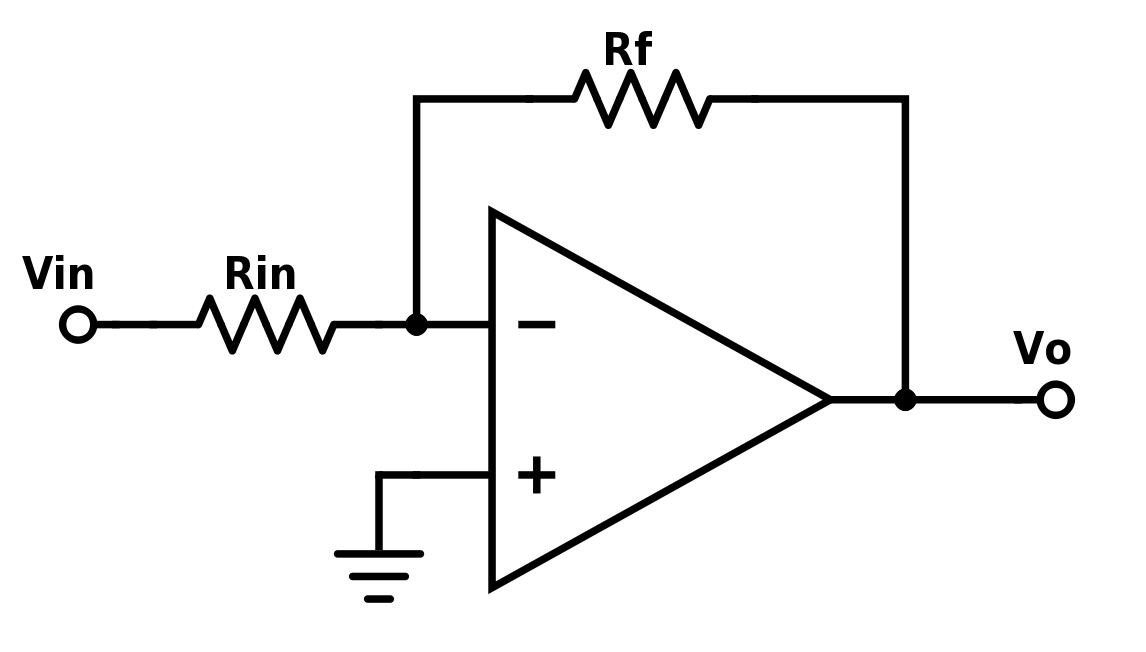
\includegraphics[scale=.15]{figures/460-17-0-INVOPAMP.png}
\caption{The circuit diagram used for the basic inverting op-amp}
\label{fig:CD_ivop}
\end{figure}

%% Here I figure we should derive the circuit and then write up generally how it works for each circuit.

\subsection{Summing}

To sum a signal with an op-amp we can input two signals into the $V_{+}$ input, this can be shown in property \ref{prop1} as we have a virtual ground at $V_+$, this means that:
\begin{align*}
    I_{out} &= I_{in}\\
    I_{out} &= I_{1} + I_{2}\\
    \frac{V_{out}}{R_f} &= -\frac{V_{1}}{R_1} -\frac{V_{2}}{R_2}\\
\Aboxed{    V_{out} &= -\left[ \frac{R_{f}}{R_1} V_1 + \frac{R_{f}}{R_2} V_2\right] }\\ \numberthis \label{eqn:sum}
\end{align*}

Equation \ref{eqn:sum} allows us to see that we will be able to directly add the voltage signals together, but there will be a scaling factor for each of the inputted signals which depends on the resistor which is placed in the path of the signal.

\begin{figure}[ht!]
\centering
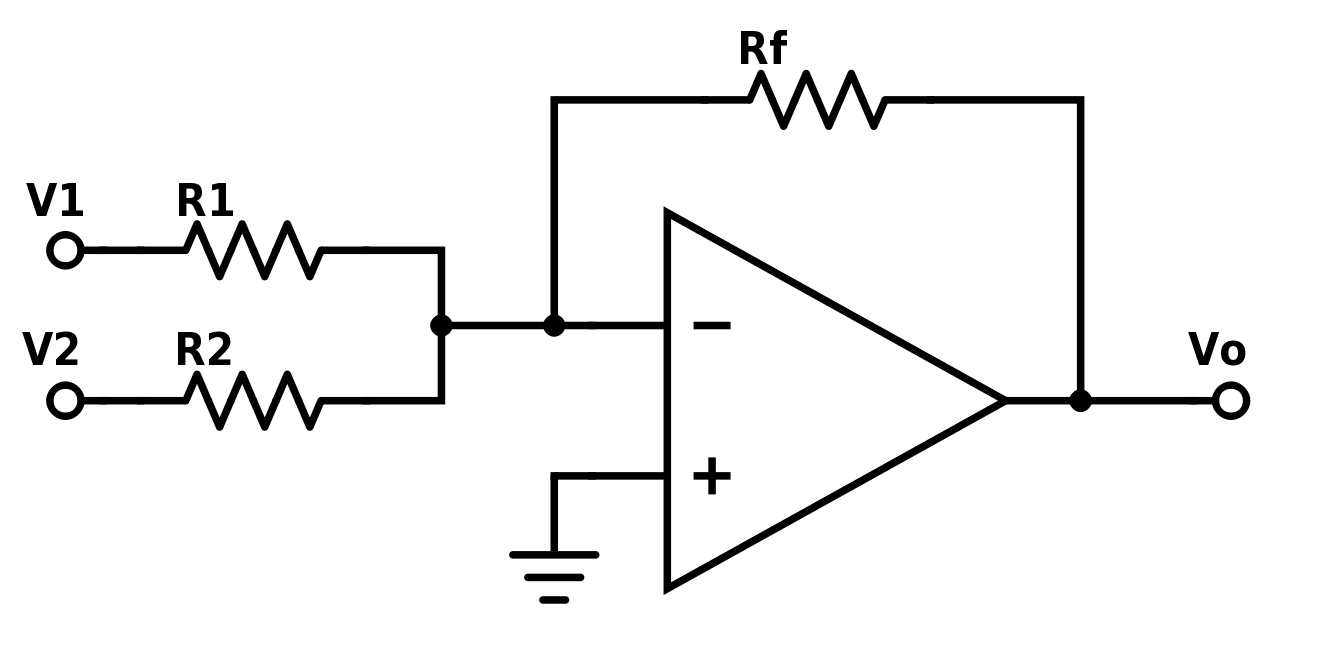
\includegraphics[scale=.15]{figures/460-17-1-Summer.png}
\caption{The circuit diagram used for summing signals from two inputs together}
\label{fig:CD_Sum}
\end{figure}


\subsection{Differentiation}

In general this op-amp has a RC network setup across the inputs which allows for the time dependant component to become significant. We can start analyzing the network:

\begin{align*}
    Q &= C V_{in}\\
\implies \frac{dQ}{dt} &= C \frac{dV_{in}}{dt}\\
\shortintertext{Noting $I_{feedback} = -V_{out}/R_f = I_{in}$ since we have a node at the input terminal:}
\implies C \frac{dV_{in}}{dt} = \frac{dQ}{dt} &= I_{in} = -\frac{V_{out}}{R_f}\\
\implies \Aboxed{ V_{out} = -R_f C \frac{dV_{in}}{dt}} \numberthis \label{eqn:diff}\\
\end{align*}

Therefore we can now see that the output voltage of the Differentiator will be directly related to the derivative of the $V_{in}$, with a scaling factor related to the two RC components. 

\begin{figure}[ht!]
\centering
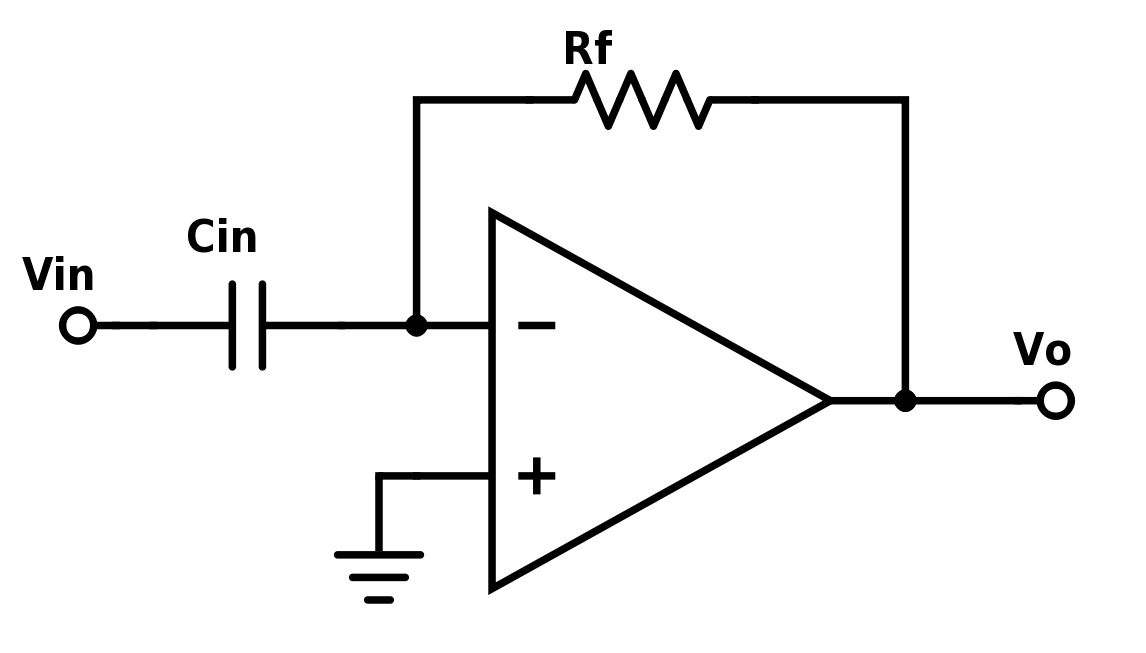
\includegraphics[scale=.15]{figures/460-17-2-Differentiator.png}
\caption{The circuit diagram used for Differentiating a signal}
\label{fig:CD_Diff}
\end{figure}

\subsection{Integration}

We now take a look at a system in which the feedback component is a capacitor, this feedback capacitor charges up as a function of it's RC time constant and hence the $V_c$ which is induced across the capacitor slowly increases and this creates a linearly increasing ramp output voltage if the input is constant. However this only occurs until the capacitor is fully charged. At this point the capacitor will become essentially an infinite resistor and this will act as if $R_f$ of an inverting op-amp is infinite. This means that gain will also be infinite.\newline

We note that the Figure \ref{fig:CD_Int} has a $C_{in}$ this is a component which is used to take out any DC current which may be introduced. Another component of the circuit diagram is the switch, which is used to create a zero gain network which will allow for the capacitor to discharge.

\begin{align*}
    Q &= C V_{in}\\
\implies \frac{dQ}{dt} &= C \frac{dV_{cap}}{dt} = C \frac{d(V_{in} + V_{out})}{dt} \\
\shortintertext{Noting $V_{in} = V_{ground} = 0 $:}
         -\frac{1}{C}\frac{dQ}{dt} &= \frac{dV_{out}}{dt} \\
\shortintertext{From principle \ref{prop2}. We can say that input impedance of the op-amp is infinite and the nodal equation at the inverting input terminal is given as:}
         I_{in} = \frac{dQ}{dt} &= \frac{V_{in}}{R_{in}}\\
                &=  C \frac{dV_{out}}{dt} \\
\implies \frac{dV_{out}}{dt} &= \frac{-1}{R_{in} C} V_{in} \numberthis \label{eqn:int_diff}\\
 \Aboxed{ V_{out} &= -\left( \frac{1}{RC} \right) \int V_{in} dt} \numberthis \label{eqn:int} \\
\end{align*}

\begin{figure}[ht!]
\centering
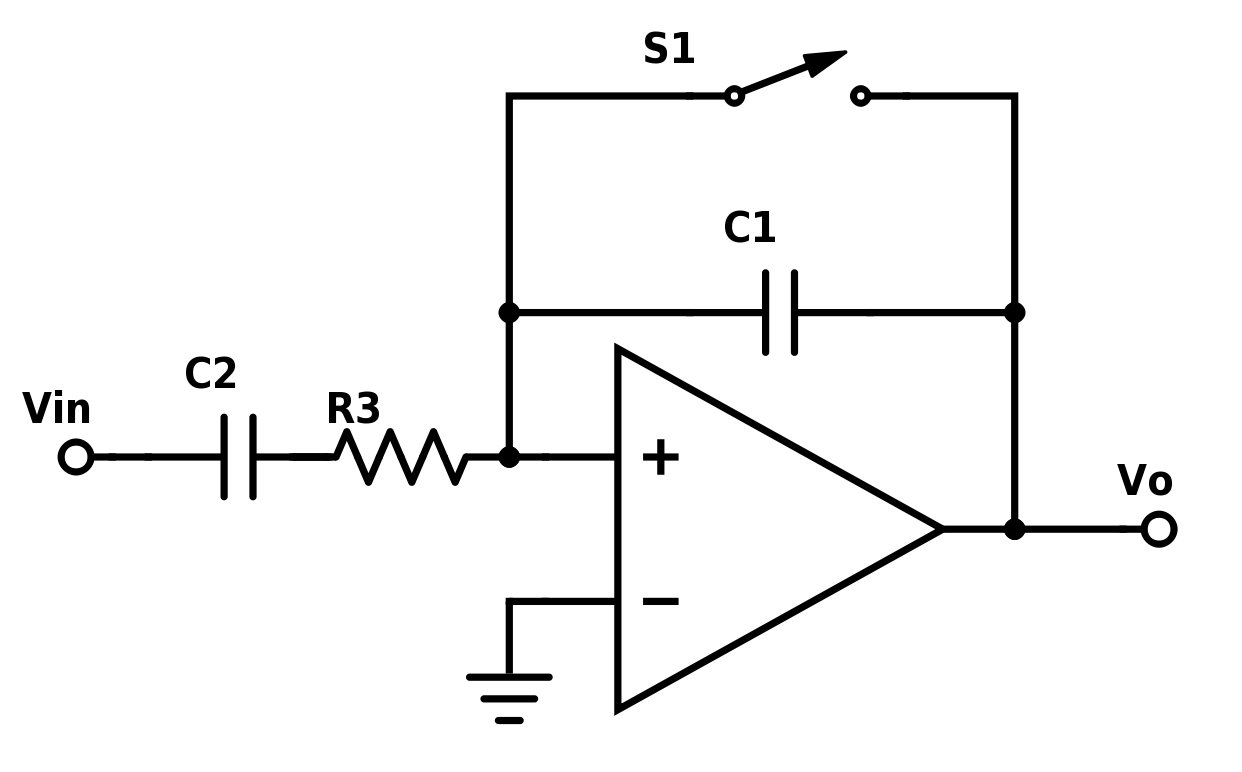
\includegraphics[scale=.18]{figures/460-17-3-Intergrator.png}
\caption{The circuit diagram used for integrating a signal}
\label{fig:CD_Int}
\end{figure}

\newpage

\subsection{Exponential}

We see that the exponential circuit above is directly related to the integration circuit. If we can ignore the potentimeter then we are able to isolate the integration section of the circuit. This can let us investigate the circuit starting with the basis of the integration circuit as in Equation \ref{eqn:int_diff}.

\begin{figure}[ht!]
\centering
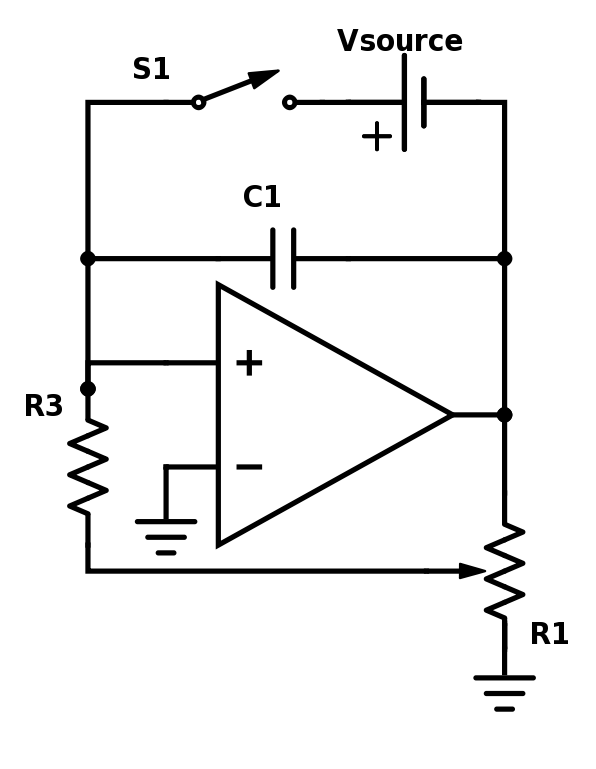
\includegraphics[scale=.2]{figures/460-17-4-Exponential.png}
\caption{The circuit diagram used for creating the solution to the exponential equation}
\label{fig:CD_Exp}
\end{figure}

Letting $R_{pot}=0$:

\begin{align*}
    \frac{dV_{out}}{dt} &= \frac{1}{R_{in} C} V_{in}\\
\shortintertext{But we note that we will feed back our voltage back into itself so $V_{out} = V_{in}$:}
    \frac{dV_{out}}{dt} &= \frac{1}{R_{in} C} V_{out}\\
    \implies V &= V_o e^{-t/RC}\\
\end{align*}

However when we add in the $R_{pot}$ the circuit becomes less simple to analyze and attempts were made to solve this circuit diagram. Taking the $R_{pot}$ to be in series with the $R_{feed}$ and simply summing them was the most obvious solution and lead to a solution of the form $V = V_o e^{-1/(R_{feed}+R_{pot})C}$. However this solution is not accurate as it alters the current flow and ignores the Voltage source. Another attempt to solve the circuit based off of current flow lead to an overall current of $I = \frac{V}{R_{pot} + R_{feed}}$ leads to a re-input voltage of:

\begin{align*}
    V_{in}  &= V_{out} -  R_{pot} \times \frac{V_{out}}{R_{pot} + R_{feed}}\\
            &= V_{out} \left(1 - \frac{R_{pot}}{R_{pot} + R_{feed}} \right)\\
            &= V_{out}\frac{R_{pot} + R_{feed} - R_{pot}}{R_{pot} + R_{feed}}\\
            &= V_{out}\frac{R_{feed}}{R_{pot} + R_{feed}} \\ 
%\implies V_{out} &= V_{in} \frac{R_{pot} + R_{feed}}{R_{feed}}\\ 
\shortintertext{Inputting this into Equation \ref{eqn:int_diff}:}
   \frac{d}{dt} V_{out} &= V_{out}  \frac{-1}{R_{in} C}\frac{R_{feed}}{R_{pot} + R_{feed}}\\
\shortintertext{This leads to a solution of the form:}
    V_{out} &= V_o e^{-\alpha t} \:,\: \alpha = \frac{R_{feed}}{(R_{pot} + R_{feed}) R_{in} C} \numberthis \label{eqn:exp_fail}\\
\end{align*}

However as we later see in Section \ref{sec:Exp} that these solutions do not work in this form. This is most likely due to an error made in this derivation based off of the treatment of the voltage source, and how the capacitor is treated. We will see that in the analysis section an experimentally verified form is discovered, with little theoretical basis. \newline

We do note however that on the input of the circuit we have $\frac{dV}{dt} = -\alpha V$ which are equivalent due to the feedback mechanisms described before. The derivative term exists form because of integrator built into the circuit and the alpha term is built into the circuit as how much feedback from the output of the integrator goes back into the input. We are unable to derive why this occurs, but we note that it will be directly related to the potentimeter's resistance as this is the term which alters the $V_{in}$ from $V_{out}$ as seen above.

\subsection{Damped Harmonic Motion}

As we can see in Figure \ref{fig:CD_HO} we are able to split up the sections of the Harmonic oscillator into several sections, each of which is described in a previous section. We note that the wave solution will be created through the feedback based in the exponential as described in the previous exponential section, and the integrator will increase the degree of it, so instead of a single exponential decay from the first order differential it will be a second order differential, which with the inverter leads to a wave solution, and with the damping will become our damped harmonic oscillator.

\begin{figure}[ht!]
\centering
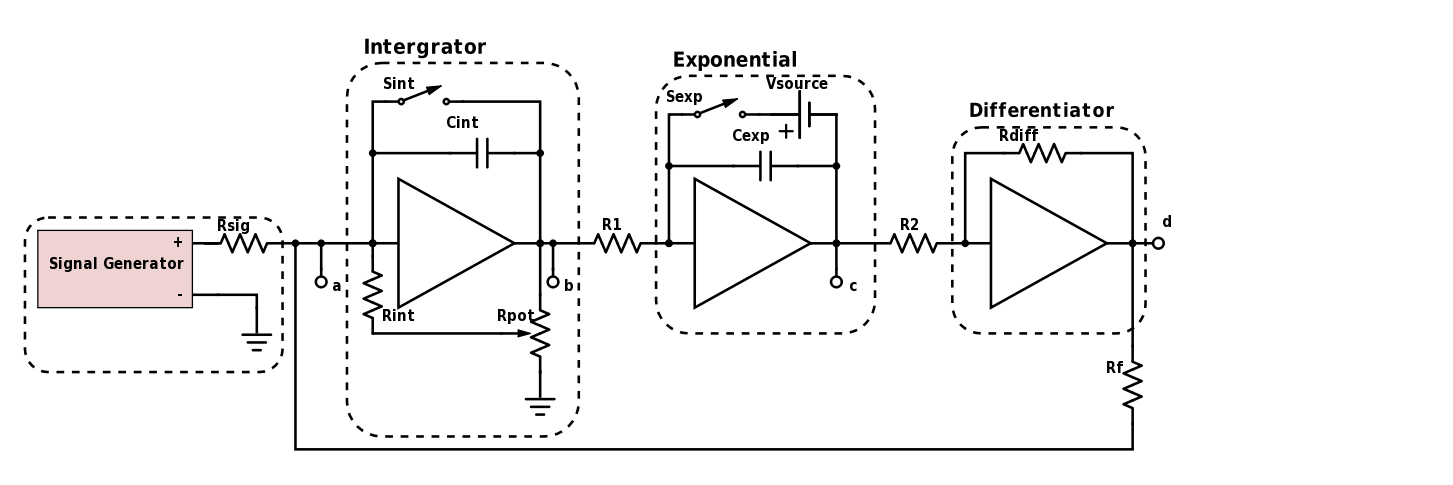
\includegraphics[scale=.43]{figures/460-17-6-Forced-HO.png}
\caption{The circuit diagram which is used for making the solution to the Damped Harmonic Oscillator, the forced section is also included}
\label{fig:CD_HO}
\end{figure}

We also note that we can pick up on sections of the solution at different points throughout the ramp as labelled. These are:
\begin{align*}
    a &= \frac{d^2 V}{dt^2} \\ 
    b &= - \frac{d V}{dt} \times \frac{1}{RC} \\ 
    c &= \frac{V}{(RC)^2} \\
    d &= - \frac{V}{(RC)^2} \\
\end{align*}

\subsection{Forced Damped Harmonic Motion}

We note that if we attempt to drive our harmonic oscillator with another wave we will be able to make it into a forced damped harmonic oscillator, this leads to the known standing wave solution and will result in different cases of dampening based off of the damping factor added in. 